\documentclass{report}

\usepackage{../../../../../LaTeX/marzstyle}

\runningheads{Privacy and Data Security}{Exercise 07}

\setcounter{chapter}{7}

\begin{document}
	\section{Differential Privacy - Theory}
	\startsection
		From the lecture we know:
		\[
			\frac{P[\fancyletter{M}(X^n) \in Y]}{P[\fancyletter{M}(\overline{X}^n) \in Y]} \ \leq \ e^{\epsilon}
		\]
		We can compute the probabilities of numerator and denumerator:
		\begin{align*}
			P[\fancyletter{M}(X^n) = 0 ] \ & = \ \delta * P[x_1 = 0] + (1-\delta) * P[R = 0] \\
			& = \ \delta * P[x_1 = 0] + \frac{1-\delta}{2} \\
			\\
			P[\fancyletter{M}(\overline{X}^n) = 0 ] \ & = \ \delta * P[\overline{x}_1 = 0] + (1-\delta) * P[R = 0] \\
			P[\overline{x}_1 = 0] \ & = \ \frac{n-1}{n} * P[x_1 = 0] + \frac{1}{n} * (1 - P[x_1 = 0]) \\
			\Rightarrow P[\fancyletter{M}(\overline{X}^n) = 0 ] \ & = \ \delta * (\frac{n-1}{n} * P[x_1 = 0] + \frac{1}{n} * (1 - P[x_1 = 0])) + \frac{1-\delta}{2}
		\end{align*}
		The fraction is greatest if the nominator is big and the denominator is small, therefore we can compute an upper bound and lower bound respectively :
		\begin{align*}
			P[\fancyletter{M}(X^n) = 0 ] \ & \leq \ \delta + \frac{1-\delta}{2} && \textit{for $P[x_1 = 0] \ = \ 1$} \\
			P[\fancyletter{M}(\overline{X}^n) = 0 ] \ & \geq \ \frac{\delta}{n} + \frac{1 - \delta}{2} && \textit{for $P[x_1 = 0] \ = \ 0$}
		\end{align*}
		Therefore we can compute the $\epsilon$:
		\begin{align*}
			e^{\epsilon} \ & \geq \ \frac{P[\fancyletter{M}(X^n) \in Y]}{P[\fancyletter{M}(\overline{X}^n) \in Y]} \ && \hspace*{-2.5cm} \leq \ \frac{\frac{1-\delta}{2}}{\frac{\delta}{n} + \frac{1 - \delta}{2}} \\
			& \Leftrightarrow \ \frac{P[\fancyletter{M}(X^n) \in Y]}{P[\fancyletter{M}(\overline{X}^n) \in Y]} \ && \hspace*{-2.5cm} \leq \ \frac{1 - \delta}{\frac{2\delta}{n} + 1 - \delta } \\
			& \Leftrightarrow && \hspace*{-2.5cm} = \ \frac{1 - \delta - \frac{2 \delta}{n} - 1 + \delta}{\frac{2 \delta}{n} + 1 - \delta} + 1 \\
			& \Leftrightarrow && \hspace*{-2.5cm} = \ \frac{-\frac{2 \delta}{n}}{\frac{2 \delta}{n} + 1 - \delta} + 1 \\
			& \Leftrightarrow && \hspace*{-2.5cm} = \ \frac{-2 \delta}{2 \delta + n - \delta n} + 1 \\
			& \Leftrightarrow && \hspace*{-2.5cm} = \ \frac{2 \delta}{2 (n-1) \delta - n} + 1 && \hspace*{-3cm} \sim 1 \ \textit{for big $n$}\\
		\end{align*}
		Because we get, that the formula is approximately around $1$, we can approximate this with $1 + x \approx e^x$. Therefore:
		\[
			\frac{2 \delta}{2 (n-1) \delta - n} + 1 \ \approx \ e^{\frac{2 \delta}{2 (n-1) \delta - n}} \ ,\textit{therefore $\epsilon \approx \frac{2 \delta}{2 (n-1) \delta - n}$  $(\approx \frac{1}{n})$ for big $n$}
		\]
	\closesection
	\newpage
	\section{Differential Privacy - Practice}
	\startsection
	The corresponding Jupyter Notebook is also handed in.
	\renewcommand{\thesubsection}{\thesection.\alph{subsection}}
		\subsection{$\epsilon$-differential histogramm on attribute \textsc{Ort}}
		\startsubsection
			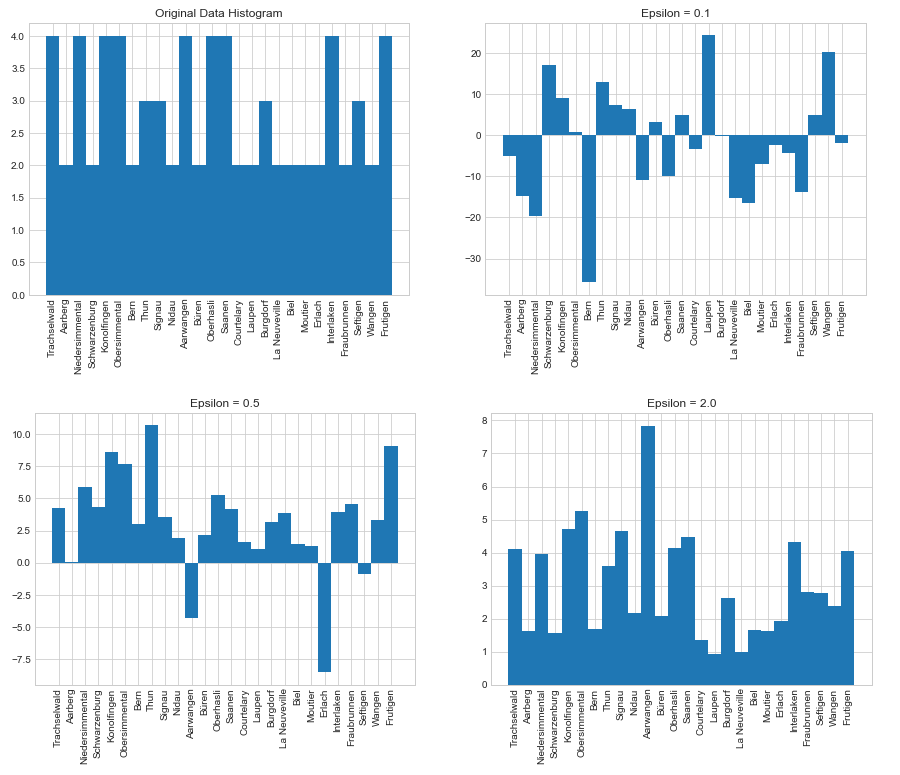
\includegraphics[scale=0.4]{DP_Orte.png}
		\closesection
		\subsection{$\epsilon$-differential histogramm on attribute \textsc{System}}
		\startsubsection
			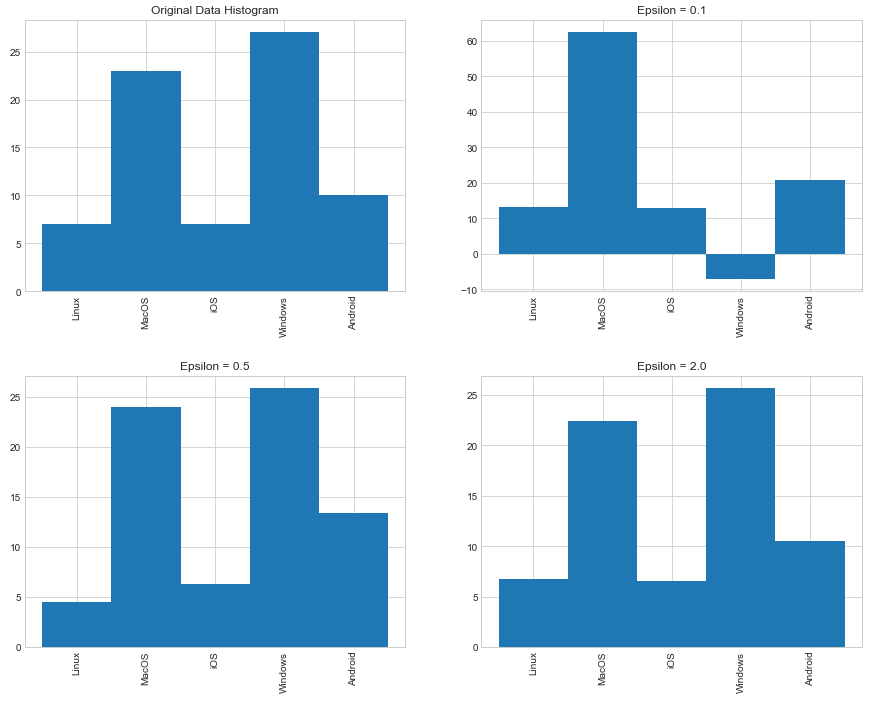
\includegraphics[scale=0.4]{DP_System.png}
		\closesection
		\subsection{$\epsilon$-differential histogramm on attribute \textsc{Points}}
		\startsubsection
			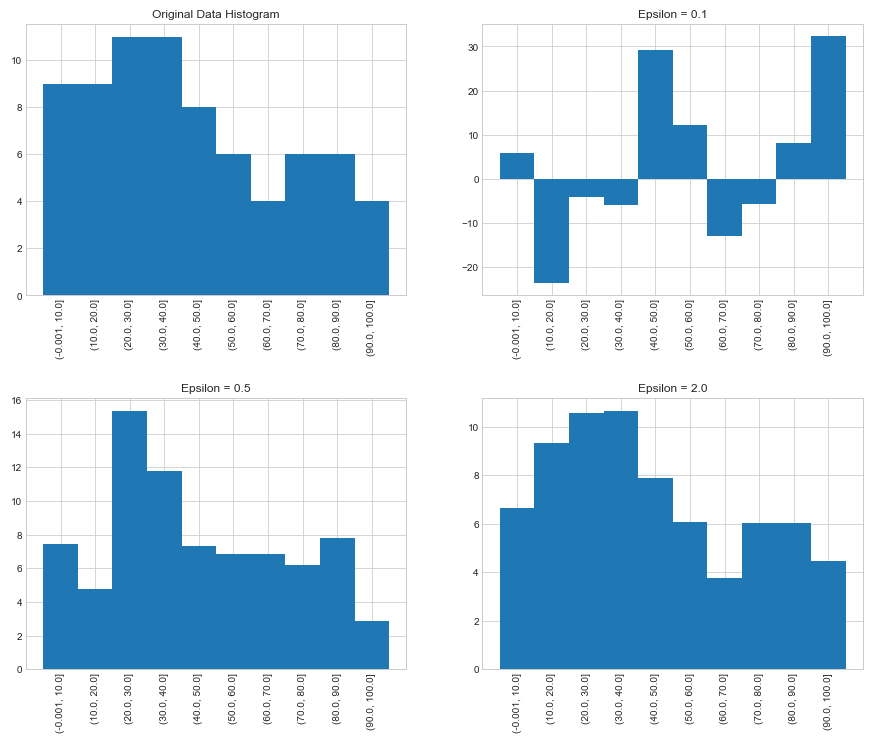
\includegraphics[scale=0.4]{DP_Points.png}
		\closesection
	The higher the $\epsilon$ value is the more do the original and the newly calculated look alike. If the $\epsilon$ is very small the histogram looks very different but it can happen that the information one can get from the histogram is not usable at all.
	\closesection
\end{document}